
\subsection{Optimal Robot Allocation}

% \newcommand{\bdag}{{\textsc DAG}}

Our proposed algorithm can be divided into two steps at the high level. 
In the first step, the algorithm conducts a \emph{generalized boustrophedon 
decomposition} for the given environment along the sweep line, 
which generates a \textit{directed acyclic graph} (DAG) representation 
of the workspace $\mathcal W$ for a given sweep schedule. 
Using the DAG, a max-flow-based algorithm is then applied to compute the 
minimum number of robots required for executing the sweep schedule, 
as well as the corresponding arrangement of robots.

\subsection{Generalized Boustrophedon Decomposition}
In solving search and coverage problems, various decomposition techniques 
have been proposed, including trapezoidal, Voronoi, boustrophedon, Morse decompositions, 
and so on \cite{huang2001optimal, choset2000coverage, breitenmoser2010voronoi, acar2002morse}.
For our robot allocation task, it is also natural to start with a decomposition 
of the environment. 
However, we need a decomposition supporting non-straight 
boundaries between the decomposed cells, created by the sweep schedule. 
For this, we propose a generalization of boustrophedon decomposition. 

Before describing the generalization of boustrophedon decomposition, 
we briefly introduce boustrophedon decomposition (readers are referred to 
\cite{choset2000coverage} for further details), which in turn is based on 
trapezoidal decomposition. The difference is that it removes the sweeping 
events that cross inner vertices. As illustrated in ~\ref{fig:trebou},
compared with trapezoidal decomposition, boustrophedon decomposition 
has fewer cells, which leads to fewer (back-and-forth) boustrophedon motions.

\begin{figure}[ht]
    \centering
    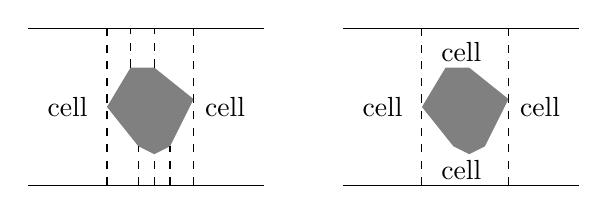
\begin{tikzpicture}
    % \fill[black] (0, 0) -- (1.9, 0.1) -- (1.3, 1) -- (1.85, 1.6) -- (0.1, 1.6) -- (0.7, 0.9) -- cycle;
    \fill[gray] (0, 0) -- (0.4, -0.5) -- (0.6, -0.6) -- (0.8, -0.5) -- (1.1, 0.1) -- (0.6, 0.5) -- (0.3, 0.5) -- cycle;
    \draw (-1, - 1) -- (2, -1); 
    \draw (-1, 1) -- (2, 1); 
    \draw[dashed] (0, -1) -- (0,1);
    \draw[dashed] (0.4, -1) -- (0.4,-0.5);
    \draw[dashed] (0.6, -1) -- (0.6,-.6);
    \draw[dashed] (0.8, -1) -- (0.8,-0.5);
    \draw[dashed] (1.1, -1) -- (1.1,1);
    \draw[dashed] (0.6, 0.5) -- (0.6,1);
    \draw[dashed] (0.3, 0.5) -- (0.3,1);
    
    \node[text=black] at (-0.5, 0.0) {cell};
    \node[text=black] at (1.5, 0.0) {cell};
    
    \fill[gray] (4, 0) -- (4.4, -0.5) -- (4.6, -0.6) -- (4.8, -0.5) -- (5.1, 0.1) -- (4.6, 0.5) -- (4.3, 0.5) -- cycle;
    
    \draw (3, - 1) -- (6, -1); 
    \draw (3, 1) -- (6, 1); 
    
    \draw[dashed] (4, -1) -- (4, 1);
    \draw[dashed] (5.1, -1) -- (5.1, 1);
    
    
    \node[text=black] at (3.5, 0.0) {cell};
    \node[text=black] at (4.5, -.8) {cell};
    \node[text=black] at (4.5, 0.7) {cell};
    \node[text=black] at (5.5, 0.0) {cell};

    \end{tikzpicture}
    \caption{[left] A trapezoidal decomposition, creating a total of $9$ cells. [right]
    Boustrophedon decomposition of the same environment, creating only $4$ cells.}
    \label{fig:trebou}
\end{figure}

We extend the boustrophedon decomposition from using only vertical sweep lines 
to allow the use of any \emph{continuous monotone sweep schedule}.
We are given a sweep schedule $P(t)$ for a workspace $\mathcal W$, 
which could take any curved form (see ~\ref{fig:Bou}).
By following the sweep schedule, it is possible to
construct a decomposition of $\mathcal W$, based on the events of cell
splitting and merging. 

\begin{figure}[ht]
    \centering
    % \includegraphics[width = .3\textwidth]{fig/bou.eps}
    \begin{overpic}[width = .4\textwidth]{chapters/sc/fig/genbou.eps}
    \put(8, 35){$v_1$}
    \put(20, 10){$v_2$}
    \put(20, 30){$v_3$}
    \put(36.5, 42){$v_4$}
    \put(55, 20){$v_5$}
    \put(50, 40){$v_6$}
    \put(80, 30){$v_7$}
    \end{overpic}
    \caption{Suppose we have a sweep schedule that sweeps the environment from left 
    to right, with curved sweep fronts. 
    The curves, as they cross critical vertices of objects, are shown as the 
    dashed lines.
    The generalized boustrophedon decomposition decomposes and $\mathcal W$ into 
    $7$ cells, $v_1\sim v_7$. 
    %
    It is important to note here that, for any continuous monotone sweep schedule,
    a decomposition can be obtained. 
    }
    \label{fig:Bou}
\end{figure}


\begin{theorem}
A sweep schedule can be organized in a DAG by the generalized boustrophedon decomposition.
\end{theorem}

\begin{proof}
Following the sweep schedule, we can conduct a generalized boustrophedon 
decomposition of the workspace $\mathcal W$. 
%
A node in the DAG will represent a cell after the decomposition, whose 
parents and children are the predecessor and successor cells along the 
sweep schedule. 

Additionally, we add a source node that links to all nodes without a parent 
and add a terminal node that links from all nodes without a child.
%
Since obstacles in the environment can contain concave vertices, we must 
consider two special cases involving concave vertices for the construction of DAG, 
as illustrated in ~\ref{fig:concave_vertices}. 
%
When a line segment of the sweep schedule ends at a concave vertex, 
the corresponding node in the DAG is linked to the terminal node $t$.
When a line segment of the sweep schedule starts at a concave vertex,
the corresponding node in the DAG is linked from the source node $s$.
In mapping these scenarios to detailed plans, it means that 
some robots will start later or end earlier compared with 
others.
% \end{remark}

\begin{figure} [ht]
    \centering
    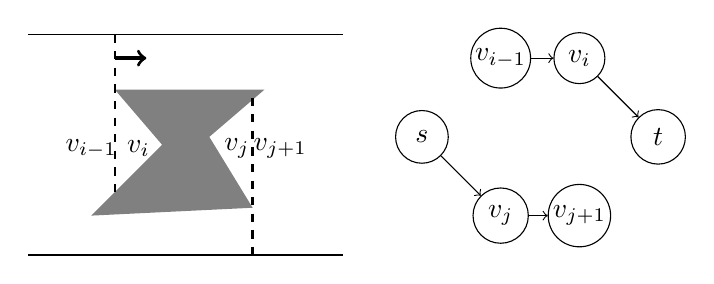
\begin{tikzpicture}
    \fill[gray] (-0.2, 0) -- (1.85, 0.1) -- (1.3, 1) -- (2.0, 1.6) -- (0.1, 1.6) -- (0.7, 0.9) -- cycle;
    \draw (-1, - 0.5) -- (3, -.5); 
    \draw (-1, 2.3) -- (3, 2.3); 

    \draw[dashed, line width=0.9pt, black] (0.1, 2.3) -- (0.1, 0.3);
    \draw[dashed, line width=0.9pt, black] (1.85, 1.5) -- (1.85, -0.5);
    
    
    \draw(-0.2, 0.85) node[text=black] { $v_{i\text{-}1}$};
    \draw(0.4, 0.85) node[text=black] {$v_i$};
    \node[text=black] at (1.65, 0.85) {$v_j$};
    \node[text=black] at (2.2, 0.85) {$v_{j\text{+}1}$};
    
    \draw(4, 1.0) node [circle, radius = 0.12, draw, inner sep=4.5](s){ $s$};
    
    \draw(5, 2.0) node [circle, radius = 0.12, draw, inner sep=0.8](vi1){ $v_{i\text{-}1}$};
    \draw(6, 2.0) node [circle, radius = 0.12, draw, inner sep=3](vi){ $v_{i}$};
    
    \draw(5, 0.0) node [circle, radius = 0.12, draw, inner sep=3](vj){ $v_{j}$};
    \draw(6, 0.0) node [circle, radius = 0.12, draw, inner sep=0.8](vj1){ $v_{j\text{+}1}$};
    
    \draw(7, 1.0) node [circle, radius = 0.12, draw, inner sep=4.5](t){ $t$};
    
    \draw[->] (vi) -- (t);
    \draw[->] (vi1) -- (vi);
    
    \draw[->] (vj) -- (vj1);
    \draw[->] (s) -- (vj);
    
    \draw[very thick, ->] (0.1, 2.0) -- (0.5,2.0);
    \end{tikzpicture}
    \caption{An example that contains two concave scenarios. As a result of the DAG construction, some robots will
    start their work at $v_j$ (by having $s$ as its parent) and some robots will end their work at $v_i$ (by having $t$ as its child).}
    \label{fig:concave_vertices}
\end{figure}
\end{proof}

% \begin{remark}



The implementation of the generalized boustrophedon decomposition is similar 
to vertical decomposition, we provide here an implementation 
Alg.~\ref{alg:genbou} adapted from \cite{lavalle2006sweepline} under the 
\emph{generation position} assumption (i.e., there are no degenerative 
settings).
%
Basically, the algorithm works by maintaining a binary search tree for 
\emph{boundary chains} representing cell boundaries. The algorithm considers 
two types of events during the sweeping process: splitting a cell into two 
cells and merging two cells into one cell.
%
Since the time cost mainly comes from maintaining the binary search tree of 
chains, with an efficient implementation, Alg.~\ref{alg:genbou} requires 
$O(n \log n)$ time, where $n$ is the complexity of the environment. 


\subsection{Reduction to Circulation with Demand}
Since we are working with \emph{monotone sweep schedules}, for any point $p$ in 
$\mathcal W$, it can only be contained in $P(t')$ for a single $t'$, i.e., each 
point $p \in \mathcal W$ is only swept once. 
%
Denote the length of the line segment where it is contained as $L$, which 
requires at least $\zeta(L)$ robots inside that segment at time $t'$
(recall that $\zeta$ is the primitive defined in Sec.~\ref{sec:sensing}).
%
For each decomposed cell, the minimum number of robots required is $\zeta(l_{max})$, where $\ell_{max}$ 
is the maximum length of the sweep line inside that cell.
%
Given a DAG $G(V,E)$ that represents the sweep schedule, the arrangement problem of the robots along the sweep line can be transformed into a network 
flow problem on the DAG.
%
For each node $v\in G$, there is a requirement of coverage for the node, 
$demand(v)$, which can be computed as $\zeta(v.\ell_{max})$.
%
Given the DAG and the demands, we are then to ``flow'' the robots through 
the schedule, allocating a certain number of robots to each decomposed cell 
along the way to satisfy these demands. 
%

Specifically, our problem may be further cast as a \emph{circulation with demand} 
problem \cite{kleinberg2006algorithm}, with the following augmentation. We replace 
each node $v$ in $G$ with two vertices $v_1$ and $v_2$ and replace every edge 
$uv$ in the previous graph with edge $u_2 v_1$, as illustrated in ~\ref{fig:flow}. 
The edge between $v_1$ and $v_2$ has flow demand of $demand(v)$. 
The following minimum circulation with demand problem is then obtained.

\begin{algorithm}[h!]
\SetKwFunction{genbou}{GenBouDecomp}
%\begin{small}
\KwData{$P(t)$: a sweep schedule. $\mathcal W$: the workspace.}
\KwResult{a DAG from the decomposition.}
\vspace{1mm}
\SetKwComment{comment}{\%}{}
\DontPrintSemicolon
\SetKw{arrival}{Arrival}

1. Separate the boundaries of obstacles into a set of \emph{monotone chains},
where each chain has the points on it \emph{arrival time} arranged in an 
increasing order.;\;
\vspace{0.5mm}
% Denote $k$ as the number of chains obtains;\;

2. $T\gets$ A binary search  tree of the chains\;
\vspace{0.5mm}

3. Construct an \emph{event array} that contains the events of the start of a chain and the end of a chain, sorted by their occurrence time during the sweep.\;
\vspace{0.5mm}

4. Iterate over the event array, which inserts and deletes chains from the binary search tree $T$, while making sure that $T$ represents the current order of the chains.\;
\vspace{0.5mm}
%\comment{\begin{footnotesize}With the general position assumption, the events comes as a paired operation for either deletion or insertion of chains \end{footnotesize}}

% When two chains are added to $T$, a cell is split into two new cells in the case of convex
% vertex or a new cell is created.  An edge from $s$ is added for a concave vertex.\;
When two chains are added to $T$, a cell is split into two new cells in the case of a convex vertex, or a new cell is created for a concave vertex, where an edge directed from $s$ is added.\;
% When two chains are removed from $T$, two cells are merged into a new cell in the case of 
% convex vertex or a cell disappears. An edge is added to $t$ for a concave vertex.\;
When two chains are removed from $T$, two cells are merged into a new cell in the case of a convex vertex or a cell disappears for a concave vertex, where an edge is added directed to $t$.\;

5. Return the DAG constructed based on $P(t)$.
%\end{small}
\caption{\protect\genbou{$P$, $\mathcal{W}$}: Generalized Boustrophedon Decomposition} 
\label{alg:genbou}
\end{algorithm}

\begin{figure}[h]
    \centering
    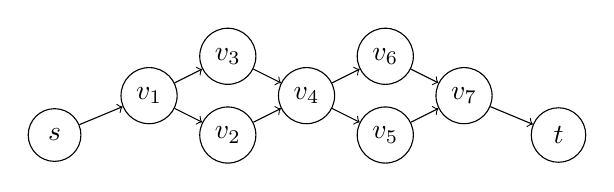
\begin{tikzpicture}
    % \node[circle](v1){$v1$};
    % \node[circle](v2){$v2$};
    % \draw[->] (v1.east) -- (v2.west);
    \draw(0,0) node [circle, radius = 0.12, draw](v1){ $v_1$};
    \draw(1, -0.5) node [circle, radius = 0.12, draw](v2){ $v_2$};
    \draw(1, 0.5) node [circle, radius = 0.12, draw](v3){ $v_3$};
    \draw(2, 0.0) node [circle, radius = 0.12, draw](v4){ $v_4$};
    \draw(3, -0.5) node [circle, radius = 0.12, draw](v5){ $v_5$};
    \draw(3, 0.5) node [circle, radius = 0.12, draw](v6){ $v_6$};
    \draw(4, 0.0) node [circle, radius = 0.12, draw](v7){ $v_7$};
    
    \draw(-1.2, -.5) node [circle, radius = 0.2, draw,inner sep=4.5](s){ $s$};
    
    \draw(5.2, -.5) node [circle, radius = 0.2, draw,inner sep=4.5](t){ $t$};
    
    \draw[->] (v1) -- (v2);
    \draw[->] (v1) -- (v3);
    \draw[->] (v2) -- (v4);
    \draw[->] (v3) -- (v4);
    \draw[->] (v4) -- (v5);
    \draw[->] (v4) -- (v6);
    \draw[->] (v5) -- (v7);
    \draw[->] (v6) -- (v7);
    
    \draw[->] (s) -- (v1);
    \draw[->] (v7) -- (t);
    \end{tikzpicture}
    \caption{The constructed DAG from the example in ~\ref{fig:Bou}}
    \label{fig:sc-DAG}
\end{figure}


\begin{algorithm}[h!]
%\begin{small}
\DontPrintSemicolon
\SetKwFunction{mindag}{MinSweepDAG}
\SetKwFunction{dflow}{MinCirculationWithDemand}
\SetKwFunction{addedge}{add\_edge}
\SetKwFunction{addvertex}{add\_vertex}
\KwData{$dag(V, E)$: the DAG obtained from \genbou. $\zeta$: the sensing requirement primitive function.}
\KwResult{$dag$: the updated $dag$ with the robot allocation information}
\vspace{0.5mm}
$G'\gets$ a new empty graph;\;
\vspace{0.5mm}

\For{$v\in dag$}{
\vspace{0.5mm}
    $G'$.\addvertex$(v_1),$ $ G'$.\addvertex($v_2$);\;
\vspace{0.5mm}
    
    $G'.$\addedge($v_1, v2$, capa=$\infty$, demand=$\zeta(v.\ell_{max})$);\;
\vspace{0.5mm}
    
    \For{$u\in dag.neighbor[v]$}{
\vspace{0.5mm}
        $G'$.\addedge($v_2$, $u$, capa=$\infty$, demand=0);\;
    }
}
\vspace{0.5mm}

\dflow($G'$);\;
\vspace{0.5mm}

\For{$v\in dag$}{
\vspace{0.5mm}
    $dag.v.guards\_num\gets$ $G'.flow[v_1][v_2]$;\;
    
\vspace{0.5mm}
    \For{$u\in dag.neighbor[v]$}{
        $dag.flow[v][u] = G'.flow[v_2][u_1]$;\;
    }
    
}


\Return{$dag$}\;

% \begin{small}

%\end{small}
\caption{\protect\mindag{$dag$, $\zeta$}{}}
\label{alg:mindag}
\end{algorithm}

\begin{figure*}[h!]
\vspace{2mm}
    \centering
    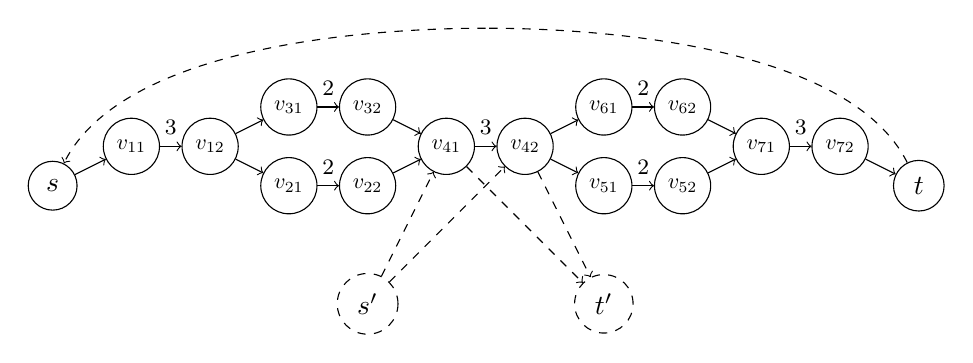
\begin{tikzpicture}[scale = 1, every node/.style={inner sep=4}]
    \draw(0,0) node [circle, draw, scale = 0.8](v11){ $v_{11}$};
    \draw(1,0) node [circle, draw, scale = 0.8](v12){ $v_{12}$};
    
    \draw(2, -0.5) node [circle, draw, scale = 0.8](v21){ $v_{21}$};
    \draw(3, -0.5) node [circle, draw, scale = 0.8](v22){ $v_{22}$};
    
    \draw(2, 0.5) node [circle, draw, scale = 0.8](v31){ $v_{31}$};
    \draw(3, 0.5) node [circle, draw, scale = 0.8](v32){ $v_{32}$};
    
    \draw(4, 0.0) node [circle, draw, scale = 0.8](v41){ $v_{41}$};
    \draw(5, 0.0) node [circle, draw, scale = 0.8](v42){ $v_{42}$};
    
    \draw(6, -0.5) node [circle, draw, scale = 0.8](v51){ $v_{51}$};
    \draw(7, -0.5) node [circle, draw, scale = 0.8](v52){ $v_{52}$};
    
    \draw(6, 0.5) node [circle, draw, scale = 0.8](v61){ $v_{61}$};
    \draw(7, 0.5) node [circle, draw, scale = 0.8](v62){ $v_{62}$};
    
    \draw(8, 0.0) node [circle, draw, scale = 0.8](v71){ $v_{71}$};
    \draw(9, 0.0) node [circle, draw, scale = 0.8](v72){ $v_{72}$};
    
    \draw(-1, -.5) node [circle, draw](s){ $s$};
    \draw(10, -.5) node [circle, draw](t){ $t$};
    
    \draw[->] (v12) -- (v21);
    \draw[->] (v12) -- (v31);
    \draw[->] (v22) -- (v41);
    \draw[->] (v32) -- (v41);
    \draw[->] (v42) -- (v51);
    \draw[->] (v42) -- (v61);
    \draw[->] (v52) -- (v71);
    \draw[->] (v62) -- (v71);
    
    \draw[->] (v11) -- node[above]{\footnotesize $3$} (v12) ;
    \draw[->] (v21) -- node[above]{\footnotesize $2$} (v22) ;
    \draw[->] (v31) -- node[above]{\footnotesize $2$} (v32) ;
    \draw[->] (v41) -- node[above]{\footnotesize $3$} (v42) ;
    \draw[->] (v51) -- node[above]{\footnotesize $2$} (v52) ;
    \draw[->] (v61) -- node[above]{\footnotesize $2$} (v62) ;
    \draw[->] (v71) -- node[above]{\footnotesize $3$} (v72) ;
    
    \draw[->] (s) -- (v11) ;
    \draw[->] (v72) -- (t) ;
    
    \draw[dashed] (t) .. controls(9, 1.5) and (5, 1.5) .. (4.5, 1.5);
    \draw[dashed,->] (4.5,1.5) .. controls(4,1.5) and (0,1.5) .. (s);
    
    \draw(3, -2) node [circle, draw, dashed] (s'){$s'$};
    \draw(6, -2) node [circle, draw, dashed] (t'){$t'$};
    
    \draw[dashed,->] (s') -- (v41);
    \draw[dashed,->] (v41) -- (t');
    
    \draw[dashed,->] (s') -- (v42);
    \draw[dashed,->] (v42) --  (t');
    
    \end{tikzpicture}
    \caption{Transform the DAG in ~\ref{fig:DAG} into a circulation with demand problem. 
    The value above each edge represents the demand of the edge, which is eliminated when it is zero.
    The source node is $s$, and the target node is $t$. $s'$ and $t'$ are the auxiliary source and target for solving the ``circulation with demand'' problem.
    Also, auxiliary edges are added between $s', t'$ and every other vertex.}
    \label{fig:sc-flow}
\end{figure*}


\begin{problem}[Minimum Circulation with Demand]
There is a graph $G(V,E)$, where $s,t$ are the source and terminal nodes. 
Every edge $uv$ in $G$ has a demand of $d(uv)$ and a capacity of $c(uv)$. 
Compute minimal network flow from $s$ to $t$ that saturates all the edge 
demands.
\end{problem}

Readers are referred to \cite{kleinberg2006algorithm} for %detailed algorithm   description and proof of correctness 
the details of the classical ``circulation with demand'' problem solution with max-flow. 

Alg.~\ref{alg:mindag} outlines the operations
used in this section. We note that the 
graph data structure needs to have the functionality of adding vertex and adding 
edge with edge demand, and $G'.flow[v_1][v_2]$ denotes the flow from $v_1$ to $v_2$ on $G'$.
% By solving the maxflow problem, we 

\subsection{The Complete Allocation Algorithm}
The overall algorithm for robot allocation is described as in Alg.~\ref{alg:overall}.
To analyze the running time of Alg.~\ref{alg:overall} for a polygonal environment, 
we denote the environment complexity (number of vertices) as $n$. 
As mentioned in the previous section, the generalized boustrophedon decomposition takes $O(n\log n)$ time. 
As the generation of a node in the DAG comes from some chain insertion or deletion events, and an event would require one vertex to happen, 
there is at most $O(n)$ decomposed cells, i.e., nodes in the DAG. 
Similarly, adding edges between nodes comes from some chain insertion or deletion events, and the number of events is at most $O(n)$. 
So, both the number of edges and the number of nodes in the DAG is $O(n)$.
Moreover, it is easy to see that the DAG is a planar graph since a node corresponds to a decomposed cell, and there is an edge between nodes only if the two corresponding cells are adjacent.
The circulation with demand problem requires solving two max-flow problems based on the DAG. 
If we use the push-relabel algorithm \cite{cheriyan1989analysis} that runs in $O(V^2\sqrt{E})$, solving the max flow for this problem will cost $O(n^{2.5})$, 
% If we use the Dinic's algorithm \cite{dinitz1970algorithm} that runs in $O(V^2E)$, solving the max flow for this problem will cost $O(n^{3})$, 
since $|V|, |E| = O(n)$.% for planar graphs. 

\begin{algorithm}[ht]
%\begin{small}
\SetKwFunction{minsweep}{MinSweep}
\KwData{$P(t)$: a sweep schedule. $\mathcal W$: a compact workspace.
$\rho_0$: required sensing probability guarantee.
% Primitive function $\zeta$ to compute the minimum number of line guards required for a continuous line segment.
}
\KwResult{$n$: the minimum number of robot guards required. $plan$: the corresponding allocation plan}%, embedded in a DAG.}
\SetKwComment{comment}{\%}{}

\vspace{1mm}
Construct $\zeta$ based the sensing model and $\rho_0$\;
\vspace{1mm}

\begin{small}
\comment{Primitive function $\zeta$ is to compute the minimum number of robots required for a continuous line segment}
\end{small}
\vspace{1mm}
$dag\leftarrow \genbou(P, {\mathcal W})$;\;

\vspace{1mm}
$dag\gets \mindag(dag, \zeta)$;\;

\vspace{1mm}
$plan\gets dag$;\;

\vspace{1mm}
\begin{small}
\comment{The plan of the robots can be constructed based on the flow on the $dag$.} 
\end{small}

\vspace{1mm}
\Return{$dag.s.guards\_num$, plan};\;
% Step 2. Construct corresponding DAG for the robot sweep schedule, as well as 
% the minimum number of robots required: $\zeta(\ell_m)$ for each cell\;

% Step 3. Run the minimum flow with demand algorithm on the transformed DAG, which results in the allocation of the robots\;
%\end{small}
\caption{\protect\minsweep{$P, {\mathcal{W}}, \rho_0$}: Computing Minimum Number of Robots for a Sweep Schedule}
\label{alg:overall}
\end{algorithm}



\begin{remark}
In the case of having a fixed number of robots, 
and the objective is to 
maximize the minimum coverage probability of a point in $\mathcal W$.
We can apply binary search on the minimum coverage probability we can guarantee, where Alg.~\ref{alg:overall} can be used to decide whether some coverage probability can be guaranteed by the fixed number of robots.
% The algorithm is detailed out in Alg.~\ref{alg:fixednum}
%\r{I think a remark is enough to say it}
\end{remark}

% \begin{algorithm}[ht]
% \begin{small}
% \SetKwFunction{maxprob}{MaxProb}
% \KwData{ $P(t)$: a sweep schedule. 
% $\mathcal W:$ a compact workspace.  $k$: the number of robots. }
% \KwResult{an allocation plan for $k$ robots to achieve 
% maximum guaranteed coverage probability, embedded in a DAG.}

% $\rho_{min}, \rho_{max}\leftarrow  0$, $1$;\;

% \While{$\rho_{max}-\rho_{min} \geq \varepsilon$}{
%     % \State Construct $\zeta$ based on $\rho_{mid}=(\rho_{min} + \rho_{max})/{2}$\\
%      $n$, $plan$ $\gets \minsweep(P, {\mathcal W}, \rho_{min})$;\;
    
%     \eIf{$n > k$}{
%          $\rho_{max} \gets \rho_{mid}$;\;
%     }{
%          $\rho_{min} \gets \rho_{mid}$;\;
%     }

% }
% \Return{$\rho_{min}$, plan}
% \end{small}
% \caption{\maxprob$(P, \mathcal{W}, k)$: Maximizing the Sensing Probability Guarantee for a Sweep Schedule with Fixed Number of Robots }
% \label{alg:fixednum}
% \end{algorithm}

